
\chapter{Detecting and injecting binaries}


In this chapter, we introduce a new algorithm to detect and record binary system in nbody simulations. With this tool, we analyse the spontaneous binary population arising in the \HubLem systems and we describe a binary injection method to complete this population to match the observations.


\minitoc

\section{A new binary detection algorithm}


\subsection{Density comparison}

The study of binary populations in nbody simulations requires an algorithm to detect binary systems and compute their characteristics. The simplest approach is to compute all star-star energies and consider bound pairs as binaries. This records a lot of ephemeral interactions, as n-body dynamics cause transient bound systems. An additional criteria is needed to assess the stability and robustness of a pair as a binary.

\begin{figure}
\begin{center}
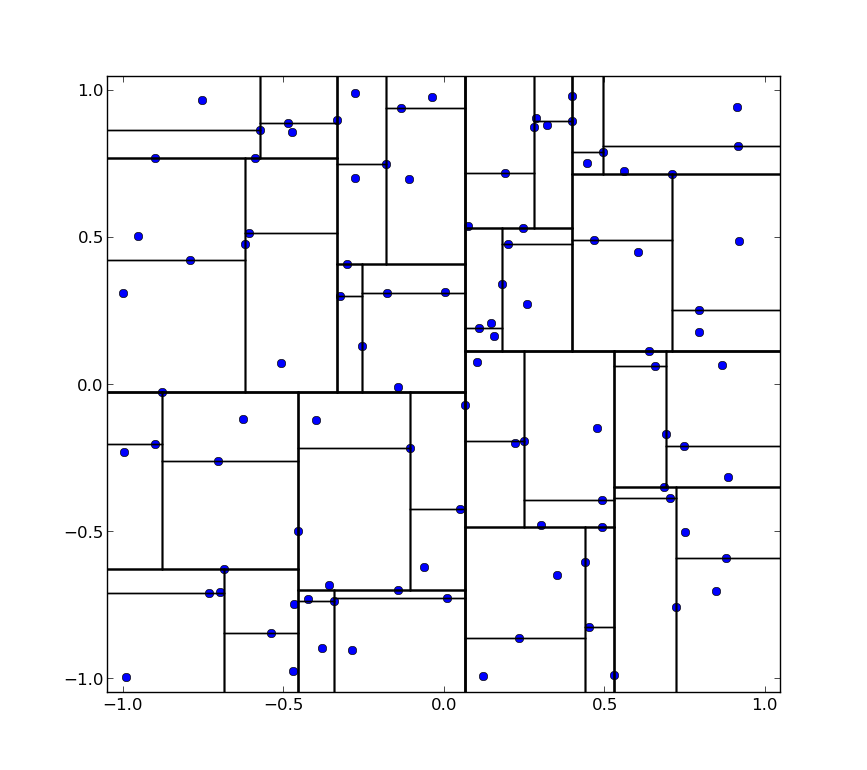
\includegraphics[width=0.6\textwidth]{Figures/5_kdtree}
\caption{Illustration of a kdtree for a random two-dimensional distribution (blue dots).}
\label{Fig:5_kdtree}
\end{center}
\end{figure}


We introduce a new algorithm based on the idea of a density threshold: binaries must be denser than their direct environment. Before describing the algorithm, we wish to emphasize the importance of neighbour searches in this kind of study. Be it to obtain bound pairs or to study said pair direct environment, the quick retrieval of neighbours is crucial to an effective algorithm.

The method described here relies on the KD-tree algorithm \citep{numericalrecipes}. While brute-force neighbour searches scale as $\propto N$, as all stars in the system have to be checked as potential neighbours, a KD tree, once built, performs neighbour searches with algorithmic complexity $\propto\log (N)$. The tree is built by sorting particles along one dimension, splitting them at the median, then sorting each branch along another dimension, splitting them again, and so on, cycling over dimensions. A two-dimensionnal example is show on Fig~\ref{Fig:5_kdtree}.





First, binary candidates are identified as negative energy pairs. The semi-major axis of the system is derived from the star motions, then a "binary density" is computed, with $a$ the binary's semi-major axis :
\begin{equation}
 \rho_{binary} = \frac{m_1 + m_2 }{4\pi a^3/3 }\, .
\end{equation}
This is then compared to the local neighbour density, defined as the cumulated mass of a fixed number $N_{nb}$ of neighbours to the pair over the spherical volume reaching to the last neighbour.
\begin{equation}
 \rho_{local} =  \frac{\sum\limits_{i=0}^{N_{nb}} m_i}{ 4 \pi r_{N_{nb}}^3 /3} .
\end{equation}


\begin{figure}
\begin{center}
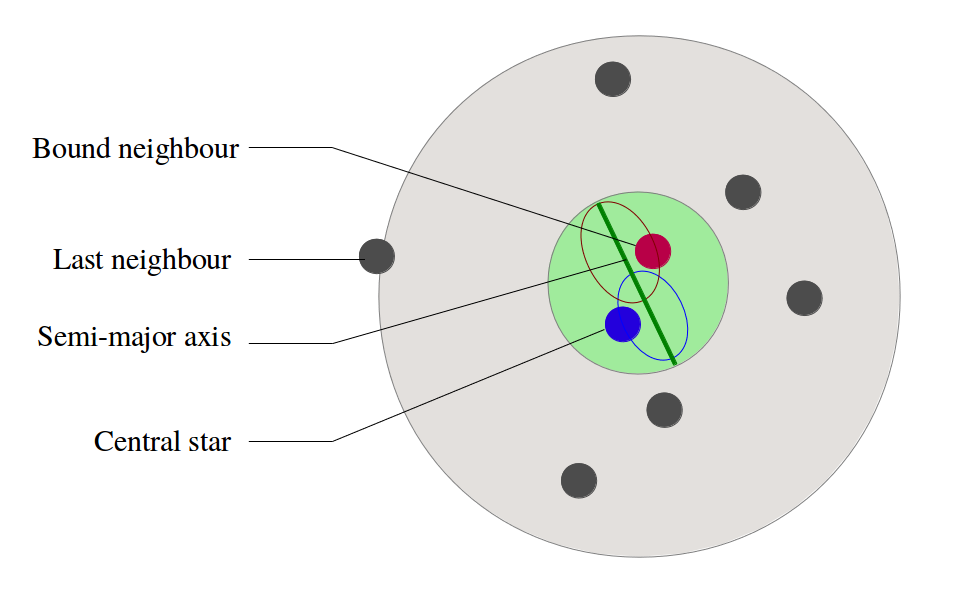
\includegraphics[width=0.6\textwidth]{Figures/5_neighbours}
\caption{Illustration of the density threshold method. The central blue stars and the red bound neighbour describe a two-body orbit shown on the figure while the green bar indicates the major-axis of the system. This defines the binary density, green sphere, while the local density is defined with the grey stars, the other neighbours. Here, $N_{nb}$ was set to 7. }
\label{Fig:5_neighbours}
\end{center}
\end{figure}




If the density ratio exceeds a threshold $D$, 
\begin{equation}
\label{Eq:density_ratio}
\frac{ \rho_{binary} }{ \rho_{local} } > D,
\end{equation}
the pair is registered as a binary.  Other authors, eg \cite{Parker2009,Lomax2015}, have used close hybrids of the criteria that we have implemented.

Stars can be found to be part of several binaries at once, which happens more often for massive stars as they clear more easily the density threshold. When that happens, the algorithm selects from such connected systems only the pairs exhibiting the lowest (most negative) binding energy.

This method has two free parameters: $N_{nb}$ and $D$. $N_{nb}$ can be set from 6 to 10 neighbours without a substantial impact on the detection. The density ratio is a more critical parameter, as if it is chosen too low, a lot of ephemeral binaries are found, while a high value picks only the closest binaries, ignoring wider, yet stable, systems.



\subsection{Choosing a density ratio}



\begin{figure}
\begin{center}
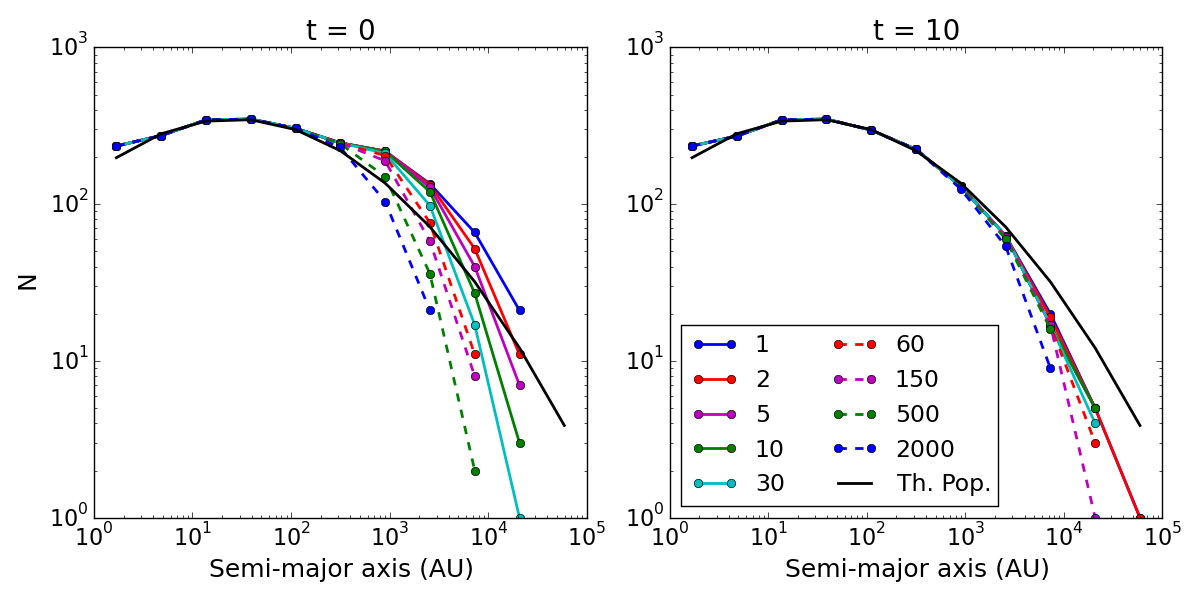
\includegraphics[width=\textwidth]{Figures/5_sm_ratios}
\caption{Semi-major axis histograms for various value of the density ratio $D$ at t=0 and 10 H.u for a 10k star King model and a binary fraction $f_b =0.3$. The injected log-normal population is shown as a black solid line.}
\label{Fig:5_sm_ratios}
\end{center}
\end{figure}



We wish to find a good compromise value for the critical density ratio $D$ that maximizes the number of detected stable binaries without collecting too much transient system. To do so, we explore the results brought by different values of $D$ in a nbody system containing binaries.

We create a virialized King model with N = 10000 stars and a binary fraction of 0.3. This means there are 2300 binaries and 5400 single stars:
\begin{equation}
f_b = \frac{N_b}{N_s + N_b} = \frac{N_b}{N-N_b} \quad \implies \quad N_b = \frac{f_b}{1+f_b} N = 2300.
\end{equation}
The binaries follow the \cite{Raghavan2010} log-normal distribution introduced in \ref{Sec:0_raghavan}. We let the system run for 10 H.u, or 12 crossing times, and write a snapshot every 0.1 H.u.

The binary detection is ran over all snapshots once per density ratio in the following list:

\begin{center}
\begin{tabular}{l|rrrrrrrrr}
\centering
D  &  2000 & 500 & 150 & 60 & 30 & 10 & 5 & 2 & 1\\ 
\end{tabular}
\end{center}

We show on Fig~\ref{Fig:5_sm_ratios} the semi-major axis distribution retrieved for various $D$ for t=0 and t=10, with the theoretical injected population as a solid black line.



\begin{figure}
\begin{center}
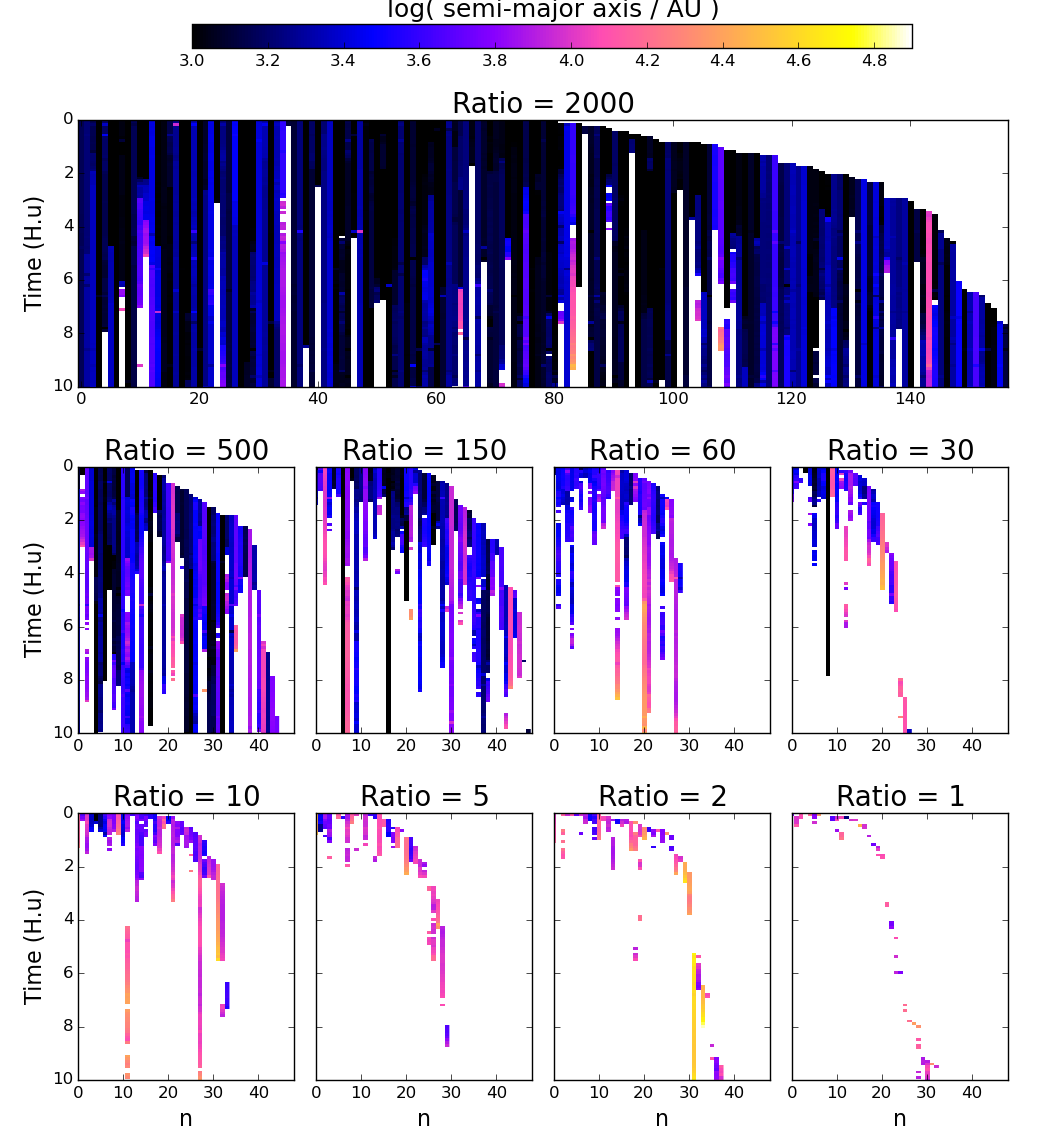
\includegraphics[width=0.9\textwidth]{Figures/5_flickering}
\caption{Visualization of the wide ($a>1000$ AU) binary population in a King model over time. Large upper panel show the evolution of all binaries detected for a density ratio $D=2000$, ordered by time of first detection. Each lower sub-panel show the new binaries detected with the new, lower, value of $D$ compared to the previous one.}
\label{Fig:5_flickering}
\end{center}
\end{figure}

Looking at the left panel, for t=0, we see all density ratios return the same population for $a < 1000$ AU, while for higher separation, there are large variations. $D = 2000$ does not detect semi-major axis larger than 3000 AU, while $D = 1$ detects $\sim$ 30 systems with $a > 10^4$ AU. After 12 crossing times, on right panels, we see the tight detected population didn't change, while all wide populations converged. The highest ratios did not undergo much change, while low ratios saw a large depletion of the population they initially returned. 

 We can say that a very high ratio only detect binaries that are garanteed to resist the dynamical processing and survive, while low ratios detect more fragile systems. How ephemeral are these latter binaries ? To evaluate the different population detected by different ratios, we show on Fig~\ref{Fig:5_flickering} the detailed evolution of the wide, $a>1000$ AU population. The large upper panel show all wide binaries evolution (time on y-axis) for $D=2000$, arranged on the x-axis by time of first detection. Each pixel column represents a binary. The smaller sub panels show, for each density ratio, the history of the binaries this ratio detected that the previous, greater ratio did not. A binary that is detected with $D=2000$ will also be detected for $D=500$ and any other lower value. Fig~\ref{Fig:5_flickering} shows what kind of binaries lowering the ratio progressively brings to the detected population. The color codes the logarithm of the semi-major axis in AU, white means the binary is not detected.

The $D=2000$ population is mainly made of stable, relatively tight binaries. About half the binaries are detected at t=0, while the others dynamically form in the system. Some are destroyed, other widened through interactions as their color bars transitions to a lighter color, sometimes after a "flickering" phase, when the detection goes on and off over successive snapshots. This is due to the binary entering a dynamical interaction with a third star or other binary, making the neighbour density undergoing spikes. This interaction leaves the binary with a weaker bound, thus higher binding energy. 

Looking at the populations brought by lower ratios, we see they are progressively wider and more transient/flickering as the ratio lowers, which is to be expected. $D=1$ only brings very ephemeral pairs, often not lasting more than a single snapshot. All ratios bring their share of transient binaries, but $D=10$ is the last to capture relevant, relatively long-lived pairs.

Extreme values of density ratios bring a large difference in the detection of large binaries, but a moderate value like $D=10$ appears the best compromise to capture the substance of a binary population.










\section{The spontaneous binary population} 




Star-star interactions which take place during the HL expansion phase speed up the internal evolution of small substructures (or, clumps). The global expansion, on the other hand, brings about correlations in phase-space coordinates and the formation of loose binary stars (see Appendix A and \citealt{Kouwenhoven2010,Moeckel2011}). We refer to that population of binary stars as {\it spontaneous} binaries in the following. There is a trade off between the creation of spontaneous binaries, and their destruction / heating when they sit near or inside a clump. Their properties as a sub-population will be addressed statistically through numerical experiments.


\subsection{Binary fraction vs primary mass}
\label{Sub:spontaneous_binaryfractions}

Several studies have found a strong correlation between the binary fraction $f_m$ and the primary mass $m$ of a binary system (for compilations, see e.g. Fig. 17 of \citealt{Bate2012} and Fig. 12 of \citealt{Raghavan2010}). Since heavy stars tend to drive the formation of clumps in HL models, by attracting stars to themselves, it is natural to expect the HL procedure to give rise to a correlation of that nature.  



\begin{figure}
\begin{center}
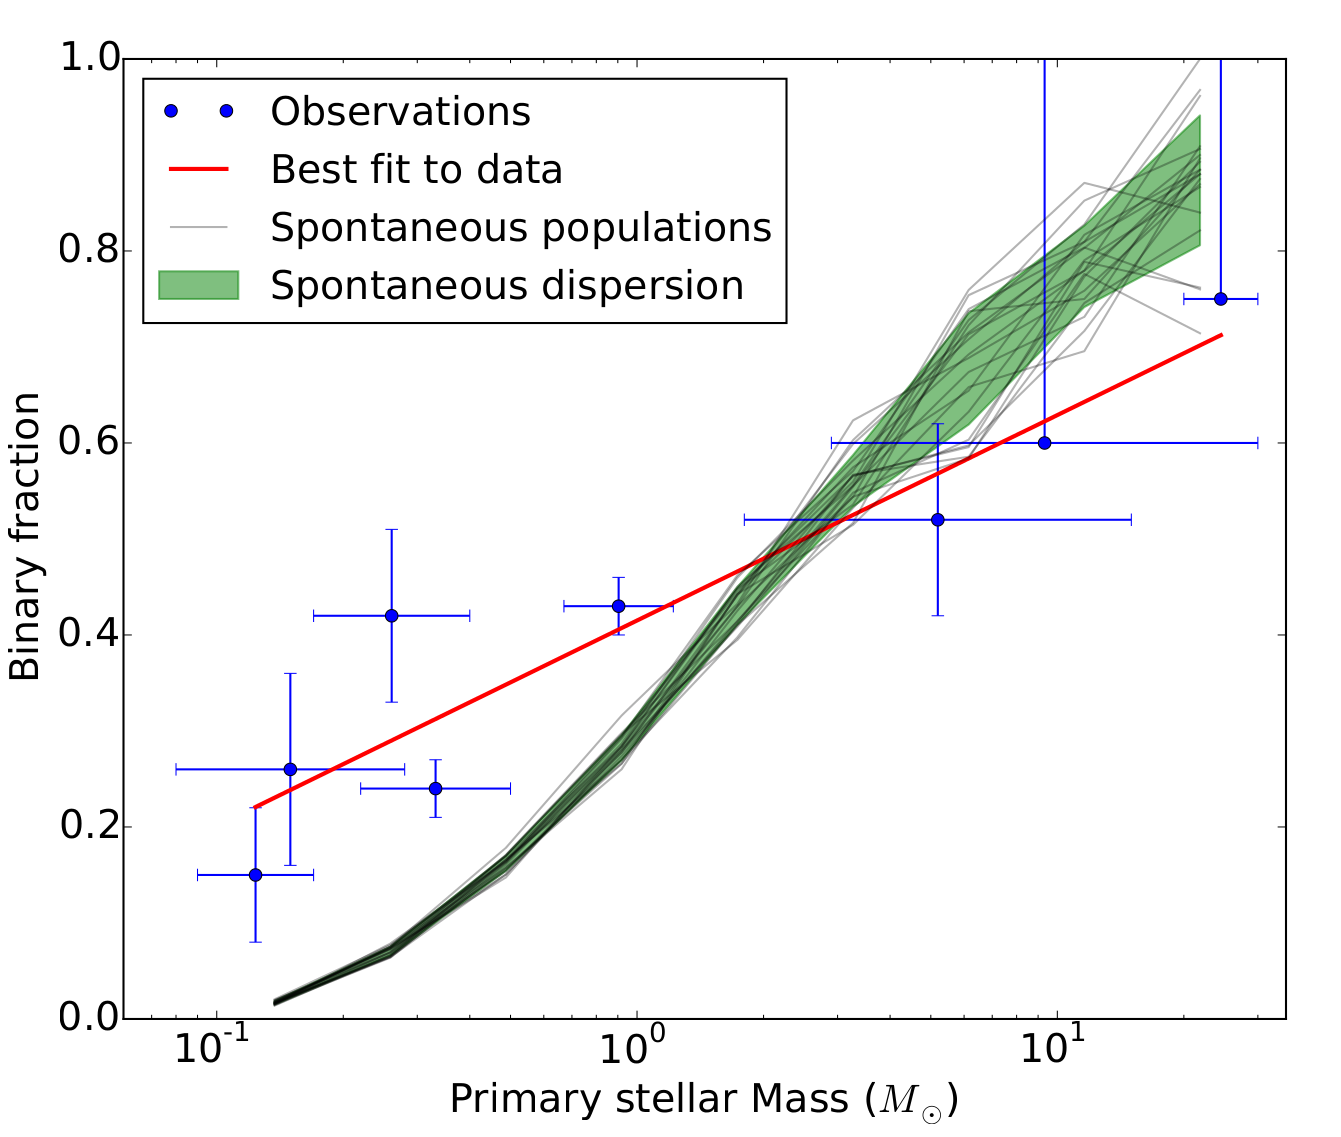
\includegraphics[width=0.7\textwidth]{Figures/5_spontaneous_primarymass}
\caption{Observational data of binary fractions (dots with uncertainties) as a function of primary mass. The data are taken from (in increasing primary mass): \protect\cite{Close2003,Basri2006,Fischer1992,Wardduong2015,Raghavan2010,Patience2002,Preibisch1999,Mason1998}. The red line is a  best-fit linear relation. The thin curves and 1-$\sigma$ dispersion shaded area are the results for a population of  spontaneous binaries obtained from HL  models.}
\label{Fig:5_spontaneous_primarymass}
\end{center}
\end{figure}




The spontaneous binary fractions found in HL models for logarithmic primary mass bins are plotted as light grey lines on Fig~\ref{Fig:5_spontaneous_primarymass}. The shaded area shows the 1-$\sigma$ dispersion for these distributions. The fraction increases rapidly  with primary mass,  and is in close agreement with the data for primaries of mass higher than 2 $M_\odot$, when $f_m$ exceeds 50\%.  However, the HL  models show  a significant deficit of low-mass primary binaries in comparison to observational data.  

The high binary fraction for heavy primaries can be explained, at least in part,  by considering the mass segregation occurring in the clumps during their formation. We shown in Chapter \ref{Chap:nbody} that massive stars tend to sink to the center of clumps. These high mass stars are more likely to capture another star to form a binary through a three-body interaction as they sit in denser environments \citep{Spitzer1987}. A heavy star also creates a deeper potential well wherein to trap a fly-by star at the on-set of HL fragmentation. There is indirect evidence for the three-body binary formation process to draw from mass-segregated clumps, because these binaries have a mean mass ratio $q = m_2/m_1$  that is significantly \textit{larger} than expected from random pairing. The mean value of $q$ for  binaries with a primary star in the range $15-30 M_\odot$  is $0.21 \pm 0.11$, whereas random pairing  yields a mass ratio of $0.02 \pm 0.02$ for that mass range. Due to mass segregation inside clumps, massive stars are more likely to pair up with moderately heavy companions rather than light ones.



\subsection{Spontaneous semi-major axis distribution}
\label{Sub:spontaneous_separations}

The distributions of semi-major axes $a$ and orbital  periods are the main parameters used to 
characterise binary populations. Up to this point, the distances were given in  computational N-body units. To convert the models to physical scales, we matched their stellar number density within the half-mass radius to that of observed clusters.  \cite{King2012a}  compiled  data for several young clusters and gave their stellar densities within half-mass radii, with high values reaching  400 stars$/pc^3$, typical of the ONC, and low-densities  of $\sim 6$ stars$/pc^3$, more akin to the Taurus region. These are the two reference values used to build up our dataset of numerical models. The time conversion gives a total duration of the simulations of 2.3 Myr for the high density clusters and 18 Myr for the low density ones.



\begin{figure}
\begin{center}
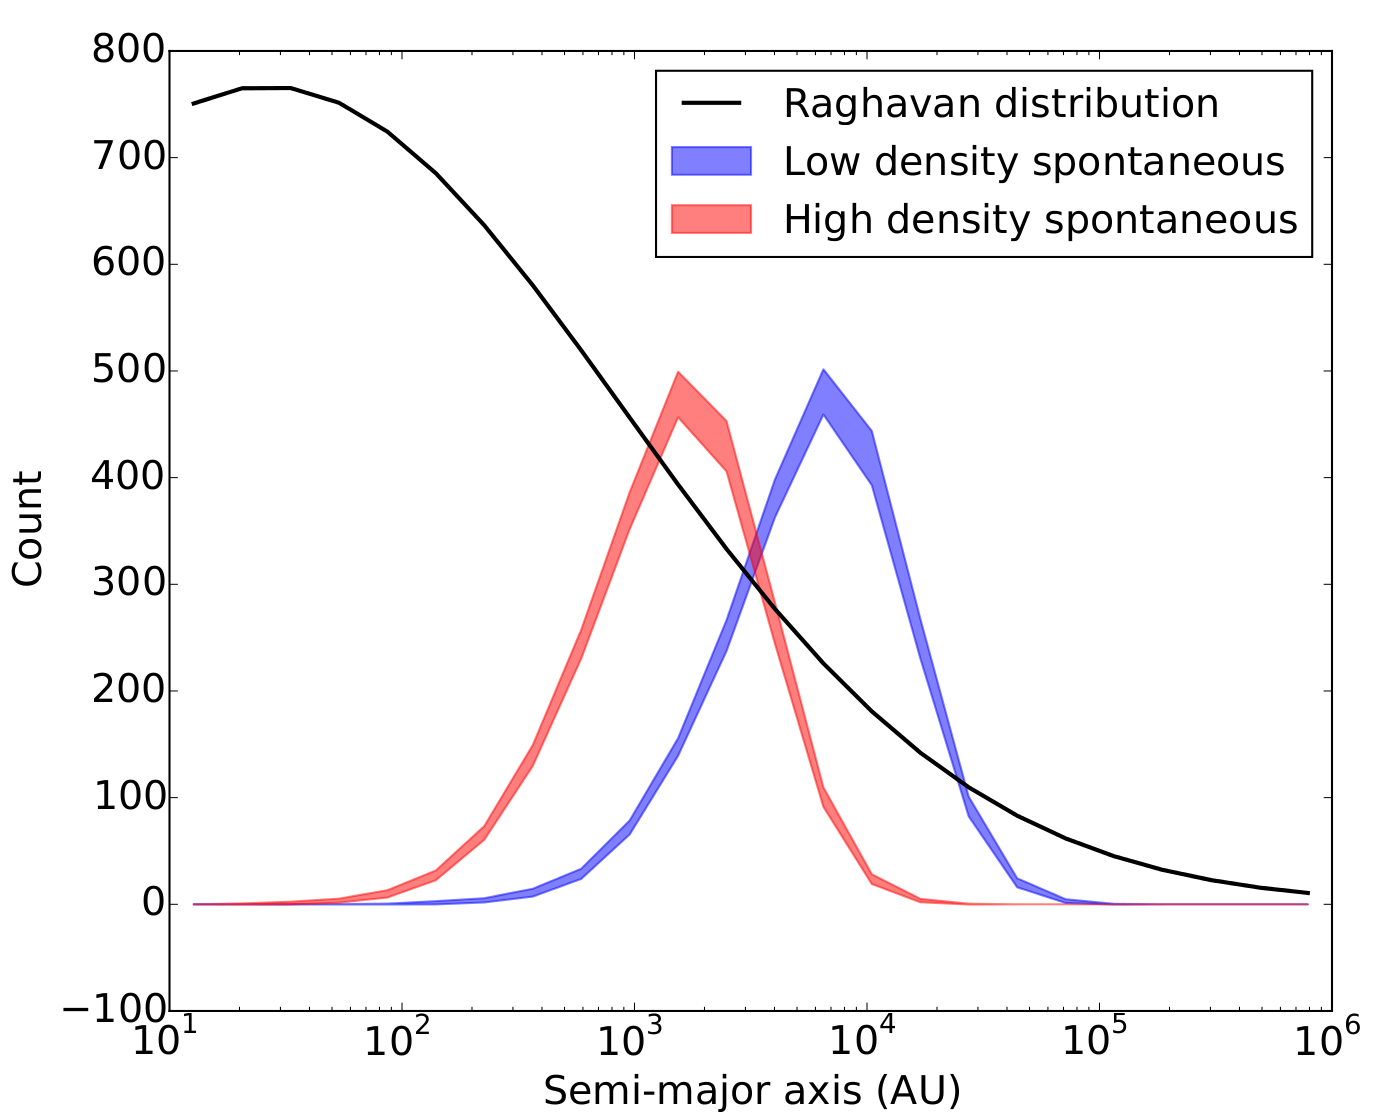
\includegraphics[width=0.7\textwidth]{Figures/5_spontaneous_smaxis}
\caption{Distribution of semi-majors axis of spontaneous binary populations for two values of stellar number density. Green curve show the canonic separation distribution from \protect\cite{Raghavan2010}. }
\label{Fig:5_spontaneous_smaxis}
\end{center}
\end{figure}


In practice the spontaneous binaries develop a bell-shaped  distribution of separation centered on $\sim 2000$ AU for a high-density HL model,  and $\sim 7000$ AU for a low-density one (see the broken curve on Fig~\ref{Fig:completed_separations}). This is much wider than the averaged value of $\sim 50$ AU for the Galactic field population \citep{DM91,raghavan2010}, where separations of $\sim 1 $ AU or lower are not uncommon. Hydrodynamical calculations by \cite{bate2012} show that orbital energy dissipated in the early stages of formation may cause binaries with an $\sim 10 $ AU  separation to shrink to $ a \sim  0.5 $ AU in the course of $t \sim 1 $ Myr. Analytical arguments by \cite{stahler2010} and \cite{korntreff2012} would have external drag forces from residual gas drive a tight binary to merge completely. \cite{kroupaburkert2001} have shown that stellar collisions  alone can not bring a narrow distribution of semi-major axes to the full width of observed values. Other studies such as \cite{parker2014}'s investigated the evolution of a binary population identical to the field but embedded in clumpy, fractal clusters \citep{goodwin2004} to test the robustness of the field population. 
A full spectrum of separations is desirable for comparison with data and theoretical models but is not a  natural outcome of the HL fragmentation. 

A trick was used to add  binaries to the fragmented HL initial conditions. We follow \cite{parker2014} to ease comparison with their setup, by supplementing the population of spontaneous binaries with one that matches the field galactic populations at small $a$. 
In doing so, we should also constrain the statistical weights with mass so as to redress the deficit of small-mass primaries (Fig.~\ref{Fig:spontaneous_binaryfractions}).



\subsection{Completing the population}
\label{Sec:Completing}

To understand the fate of a binary population in a young cluster, one needs a proper and realistic binary population. [ talk about parker, meyer, etc ]

In a recent work by \cite{parker2014}, in which the author investigated the fate of a binary population in a fractally substructured cluster, the binary population injected in the system has a varying binary fraction depending on the primary mass. Following the trend illustrated in section~\ref{Sec:SpontBinFrac}, the binary fraction increases with primary mass and fits the observations. We wish to have such a population in our fragmented cluster, however, as shown on Fig~\ref{Fig:binaryfractions} and Fig~\ref{Fig:spontaneousseparations}, the spontaneous population shows a deficit of low-mass primary, short separations binaries.

These missing binaries can be injected in the system to complete the spontaneous population and reconstitute a realistic, observations fitting population. The addition of new binaries is not straightforward, as the spatial coordinates of stars in a HL fragmented system are not under our direct control and are determined by the preceding expansion. A coherent method is to build the binary population to be injected in the system \textit{before} the expansion, and placing each binary in the initial uniform sphere as a single point bearing the mass of the two components. The HL expansion is then performed, leading to the fragmented configuration. Only then are these fused binaries split in two components with the relative positions and velocities matching their orbital parameters.

However, this implies the HL fragmentation occurs with less particles than intended in the full system, thus forming less spontaneous pairs. Furthermore, many of these spontaneous pairs form with at least one fused binary as a component, meaning they will be destroyed as this component splits into the binary it was intended to be. The proper quantity and distribution of binaries to inject is complex and dependant on several parameters: total N, HL parameter, mass function. Details on this process can be found in Dorval (2016,in prep.).


\begin{figure}
\begin{center}
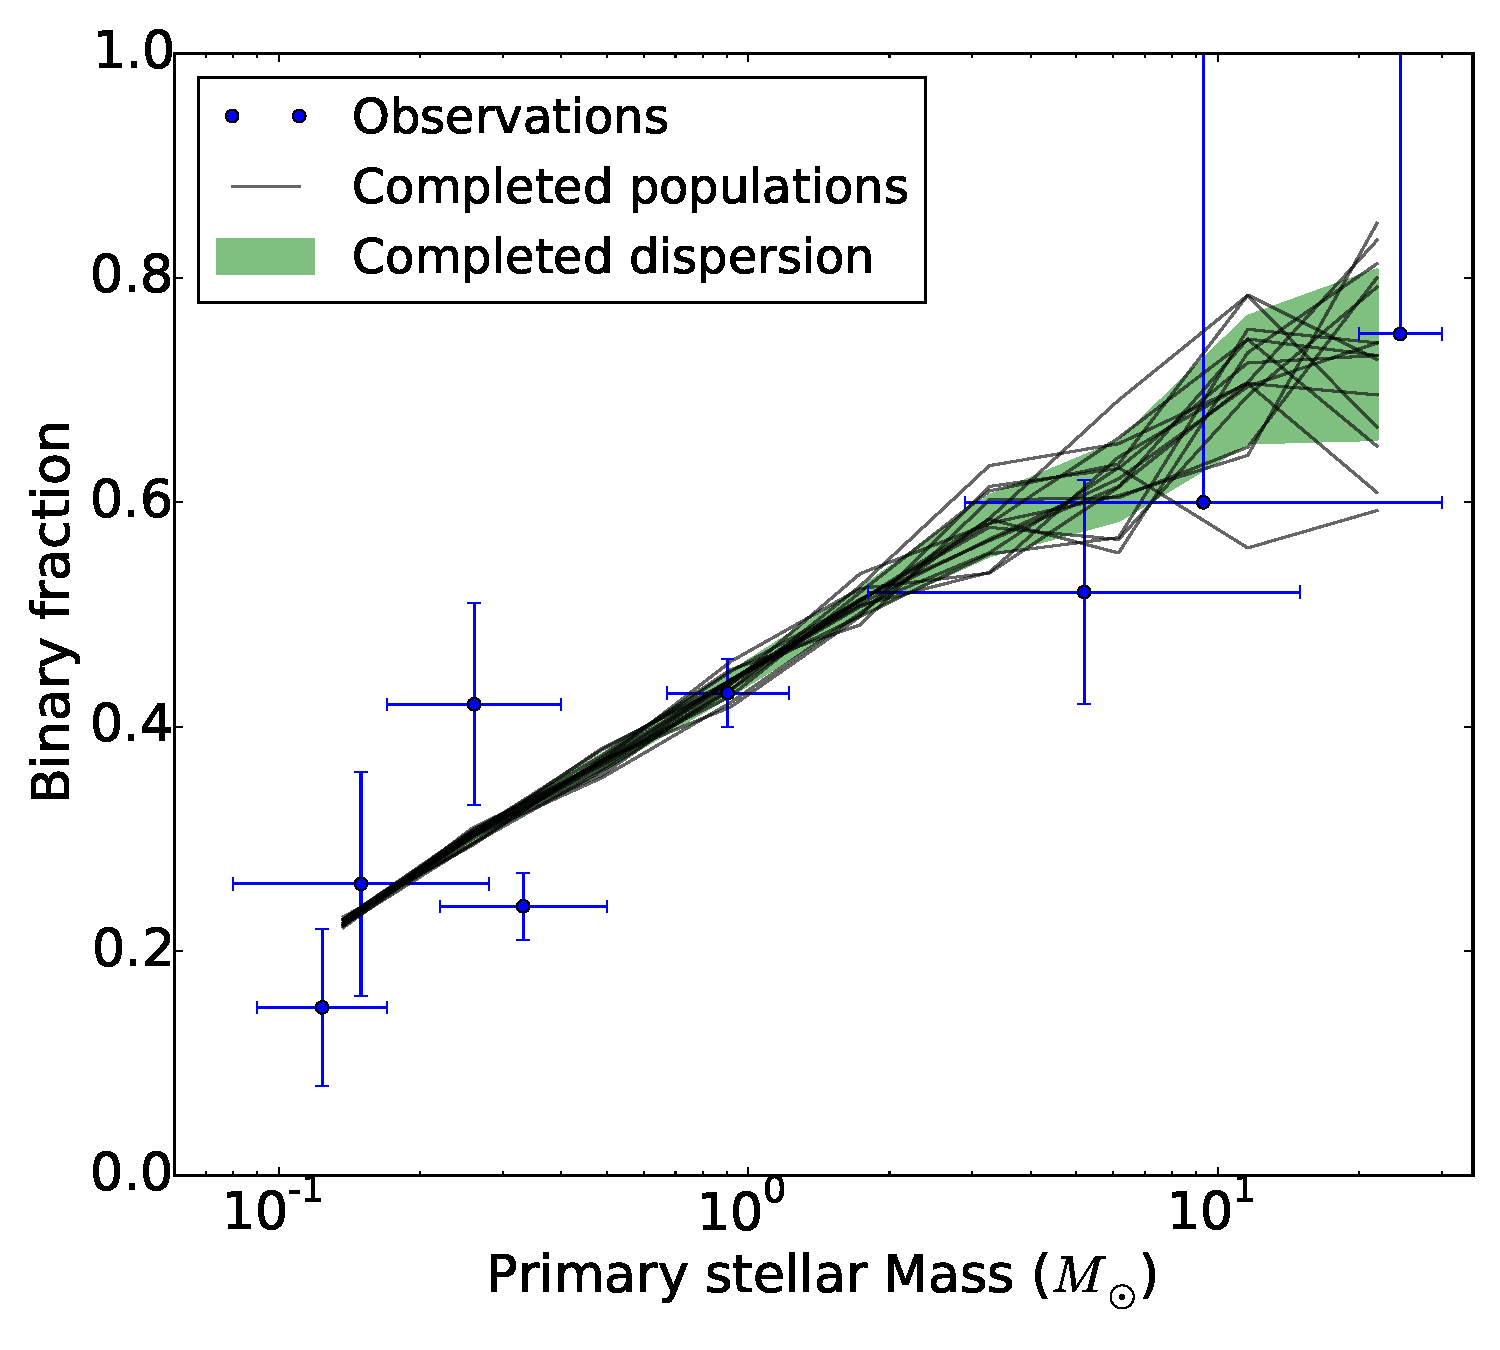
\includegraphics[width=0.7\textwidth]{Figures/5_completed_primarymass}
\caption{ Binary fraction as a function of primary mass for 20 20k particles models. Additional binaries were injected to complete the spontaneous population.}
\label{Fig:5_completed_primarymass}
\end{center}
\end{figure}

This was performed on 20 models, bearing the same characteristics than in section \ref{Sec:Spont}. The resulting binary fraction vs primary mass distribution is shown on Fig~\ref{Fig:5_completed_primarymass}. The deficit of low-mass primaries was bridged, whereas the high-mass primary binary fraction was slightly reduced. This was due to spontaneous high-mass primary binaries having a fused binary component and being destroyed at splitting. No massive binaries were introduced to compensate this, as the effect is small and the higher the spontaneous fraction, the harder it is to increase it by injecting new binaries.

As shown on Fig~\ref{Fig:5_spontaneous_smaxis}, spontaneous population exhibits a lack of small separation binaries that needs to be filled to obtain a completed distribution closer to the reality of the observed field population from \cite{Raghavan2010} that we use as a reference. We show on Fig~\ref{Fig:5_completed_smaxis} in short-dashed green the full spontaneous completion for the fragmented, before the splitting occurs. Not considering spontaneous binaries set not to survive the splitting (that is the ones with at least a fused binary as a component), we can correct the theoretical distribution by substracting the pre-existing population. This distribution is shown in long-dashed blue. The resulting distribution of semi-major axis in the system after splitting is shown in red, the theoretical distribution with a poissonian deviation is shown as a grey area.

The completed population has an excess of $\sim 10^4$ AU binaries, but a deficit of wider systems. The excess is due to the pre-existing spontaneous binaries and is hardly fixable. The "wide-axis" deficit, meaning binaries with a semi-major axis of $\sim 10^5$ AU were not found in the system,  as such systems cannot exist given the local stellar density. The low density models were used for Fig~\ref{Fig:5_completed_smaxis}, thus the mean stellar density is of 6 stars$/pc^3$. A quick calculation gives a mean distance between stars of $\sim 10^5$ AU in such an environment, making binaries this wide if not impossible, at least extremely short-lived and undetectable.

While Hubble-Lemaitre fragmentation allows to obtain a self-consistent phase space distribution for a substructured model, the population completion presented here preserves this consistency by taking into account naturally occuring multiple systems, while allowing the user to inject a realistic binary population.



\begin{figure}
\begin{center}
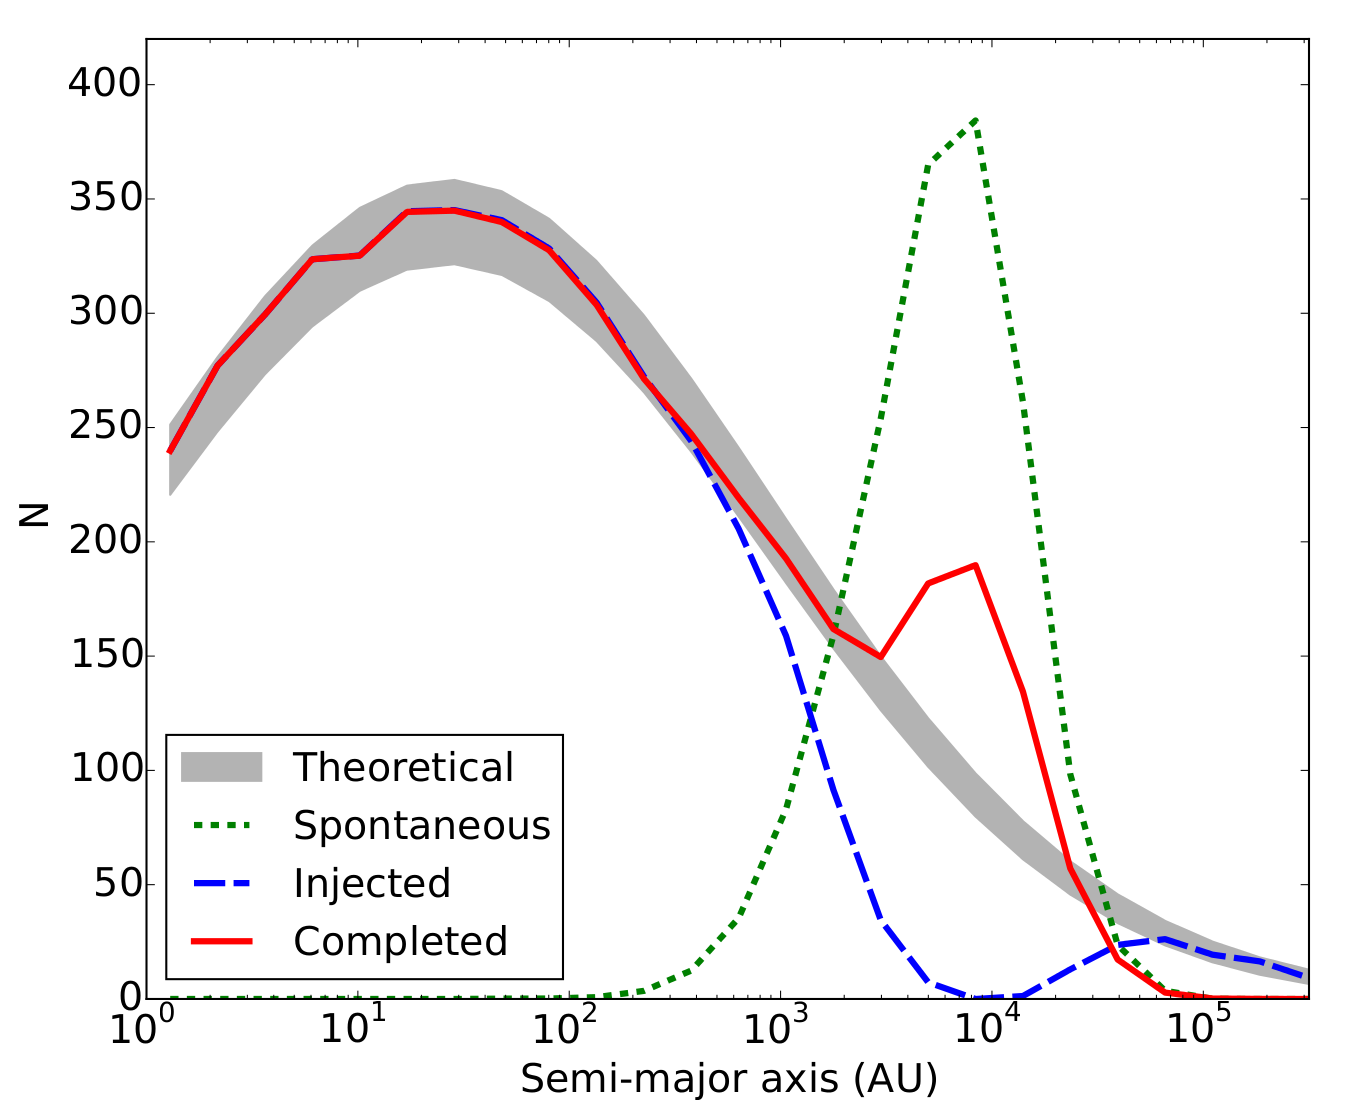
\includegraphics[width=0.7\textwidth]{Figures/5_completed_smaxis}
\caption{ Distribution histogram of binary semi-major axis for the completion of a population in a low density model. Spontaneous binaries before splitting are shown in short-dashed green, the population injected in the system in long-dashed blue and the resulting measured distribution in the completed system in red. The theoretical separation distribution from \protect\cite{Raghavan2010} is shown as a grey area, taking into account poisson dispersion.}
\label{Fig:5_completed_smaxis}
\end{center}
\end{figure}

